% Options for packages loaded elsewhere
\PassOptionsToPackage{unicode}{hyperref}
\PassOptionsToPackage{hyphens}{url}
\documentclass[
]{article}
\usepackage{xcolor}
\usepackage[margin=1in]{geometry}
\usepackage{amsmath,amssymb}
\setcounter{secnumdepth}{-\maxdimen} % remove section numbering
\usepackage{iftex}
\ifPDFTeX
  \usepackage[T1]{fontenc}
  \usepackage[utf8]{inputenc}
  \usepackage{textcomp} % provide euro and other symbols
\else % if luatex or xetex
  \usepackage{unicode-math} % this also loads fontspec
  \defaultfontfeatures{Scale=MatchLowercase}
  \defaultfontfeatures[\rmfamily]{Ligatures=TeX,Scale=1}
\fi
\usepackage{lmodern}
\ifPDFTeX\else
  % xetex/luatex font selection
\fi
% Use upquote if available, for straight quotes in verbatim environments
\IfFileExists{upquote.sty}{\usepackage{upquote}}{}
\IfFileExists{microtype.sty}{% use microtype if available
  \usepackage[]{microtype}
  \UseMicrotypeSet[protrusion]{basicmath} % disable protrusion for tt fonts
}{}
\makeatletter
\@ifundefined{KOMAClassName}{% if non-KOMA class
  \IfFileExists{parskip.sty}{%
    \usepackage{parskip}
  }{% else
    \setlength{\parindent}{0pt}
    \setlength{\parskip}{6pt plus 2pt minus 1pt}}
}{% if KOMA class
  \KOMAoptions{parskip=half}}
\makeatother
\usepackage{color}
\usepackage{fancyvrb}
\newcommand{\VerbBar}{|}
\newcommand{\VERB}{\Verb[commandchars=\\\{\}]}
\DefineVerbatimEnvironment{Highlighting}{Verbatim}{commandchars=\\\{\}}
% Add ',fontsize=\small' for more characters per line
\usepackage{framed}
\definecolor{shadecolor}{RGB}{248,248,248}
\newenvironment{Shaded}{\begin{snugshade}}{\end{snugshade}}
\newcommand{\AlertTok}[1]{\textcolor[rgb]{0.94,0.16,0.16}{#1}}
\newcommand{\AnnotationTok}[1]{\textcolor[rgb]{0.56,0.35,0.01}{\textbf{\textit{#1}}}}
\newcommand{\AttributeTok}[1]{\textcolor[rgb]{0.13,0.29,0.53}{#1}}
\newcommand{\BaseNTok}[1]{\textcolor[rgb]{0.00,0.00,0.81}{#1}}
\newcommand{\BuiltInTok}[1]{#1}
\newcommand{\CharTok}[1]{\textcolor[rgb]{0.31,0.60,0.02}{#1}}
\newcommand{\CommentTok}[1]{\textcolor[rgb]{0.56,0.35,0.01}{\textit{#1}}}
\newcommand{\CommentVarTok}[1]{\textcolor[rgb]{0.56,0.35,0.01}{\textbf{\textit{#1}}}}
\newcommand{\ConstantTok}[1]{\textcolor[rgb]{0.56,0.35,0.01}{#1}}
\newcommand{\ControlFlowTok}[1]{\textcolor[rgb]{0.13,0.29,0.53}{\textbf{#1}}}
\newcommand{\DataTypeTok}[1]{\textcolor[rgb]{0.13,0.29,0.53}{#1}}
\newcommand{\DecValTok}[1]{\textcolor[rgb]{0.00,0.00,0.81}{#1}}
\newcommand{\DocumentationTok}[1]{\textcolor[rgb]{0.56,0.35,0.01}{\textbf{\textit{#1}}}}
\newcommand{\ErrorTok}[1]{\textcolor[rgb]{0.64,0.00,0.00}{\textbf{#1}}}
\newcommand{\ExtensionTok}[1]{#1}
\newcommand{\FloatTok}[1]{\textcolor[rgb]{0.00,0.00,0.81}{#1}}
\newcommand{\FunctionTok}[1]{\textcolor[rgb]{0.13,0.29,0.53}{\textbf{#1}}}
\newcommand{\ImportTok}[1]{#1}
\newcommand{\InformationTok}[1]{\textcolor[rgb]{0.56,0.35,0.01}{\textbf{\textit{#1}}}}
\newcommand{\KeywordTok}[1]{\textcolor[rgb]{0.13,0.29,0.53}{\textbf{#1}}}
\newcommand{\NormalTok}[1]{#1}
\newcommand{\OperatorTok}[1]{\textcolor[rgb]{0.81,0.36,0.00}{\textbf{#1}}}
\newcommand{\OtherTok}[1]{\textcolor[rgb]{0.56,0.35,0.01}{#1}}
\newcommand{\PreprocessorTok}[1]{\textcolor[rgb]{0.56,0.35,0.01}{\textit{#1}}}
\newcommand{\RegionMarkerTok}[1]{#1}
\newcommand{\SpecialCharTok}[1]{\textcolor[rgb]{0.81,0.36,0.00}{\textbf{#1}}}
\newcommand{\SpecialStringTok}[1]{\textcolor[rgb]{0.31,0.60,0.02}{#1}}
\newcommand{\StringTok}[1]{\textcolor[rgb]{0.31,0.60,0.02}{#1}}
\newcommand{\VariableTok}[1]{\textcolor[rgb]{0.00,0.00,0.00}{#1}}
\newcommand{\VerbatimStringTok}[1]{\textcolor[rgb]{0.31,0.60,0.02}{#1}}
\newcommand{\WarningTok}[1]{\textcolor[rgb]{0.56,0.35,0.01}{\textbf{\textit{#1}}}}
\usepackage{graphicx}
\makeatletter
\newsavebox\pandoc@box
\newcommand*\pandocbounded[1]{% scales image to fit in text height/width
  \sbox\pandoc@box{#1}%
  \Gscale@div\@tempa{\textheight}{\dimexpr\ht\pandoc@box+\dp\pandoc@box\relax}%
  \Gscale@div\@tempb{\linewidth}{\wd\pandoc@box}%
  \ifdim\@tempb\p@<\@tempa\p@\let\@tempa\@tempb\fi% select the smaller of both
  \ifdim\@tempa\p@<\p@\scalebox{\@tempa}{\usebox\pandoc@box}%
  \else\usebox{\pandoc@box}%
  \fi%
}
% Set default figure placement to htbp
\def\fps@figure{htbp}
\makeatother
\setlength{\emergencystretch}{3em} % prevent overfull lines
\providecommand{\tightlist}{%
  \setlength{\itemsep}{0pt}\setlength{\parskip}{0pt}}
\usepackage{ctex}
\usepackage{amsmath}
\usepackage{bookmark}
\IfFileExists{xurl.sty}{\usepackage{xurl}}{} % add URL line breaks if available
\urlstyle{same}
\hypersetup{
  pdftitle={R作业2},
  pdfauthor={laijr},
  hidelinks,
  pdfcreator={LaTeX via pandoc}}

\title{R作业2}
\author{laijr}
\date{2026/4/16}

\begin{document}
\maketitle

题目1:离散分布随机数生成与频率比较

\begin{Shaded}
\begin{Highlighting}[]
\FunctionTok{set.seed}\NormalTok{(}\DecValTok{1}\NormalTok{)}

\NormalTok{vals  }\OtherTok{\textless{}{-}} \DecValTok{1}\SpecialCharTok{:}\DecValTok{5}
\NormalTok{probs }\OtherTok{\textless{}{-}} \FunctionTok{c}\NormalTok{(}\FloatTok{0.15}\NormalTok{, }\FloatTok{0.25}\NormalTok{, }\FloatTok{0.30}\NormalTok{, }\FloatTok{0.20}\NormalTok{, }\FloatTok{0.10}\NormalTok{)}
\NormalTok{n     }\OtherTok{\textless{}{-}} \DecValTok{1200}

\NormalTok{x }\OtherTok{\textless{}{-}} \FunctionTok{sample}\NormalTok{(vals, }\AttributeTok{size =}\NormalTok{ n, }\AttributeTok{replace =} \ConstantTok{TRUE}\NormalTok{, }\AttributeTok{prob =}\NormalTok{ probs)}

\FunctionTok{par}\NormalTok{(}\AttributeTok{mfrow =} \FunctionTok{c}\NormalTok{(}\DecValTok{1}\NormalTok{, }\DecValTok{2}\NormalTok{))}

\CommentTok{\# 散点图}
\FunctionTok{plot}\NormalTok{(}\DecValTok{1}\SpecialCharTok{:}\NormalTok{n, x,}
     \AttributeTok{pch  =} \StringTok{"."}\NormalTok{, }\AttributeTok{cex =} \FloatTok{1.5}\NormalTok{,}
     \AttributeTok{col  =} \StringTok{"steelblue"}\NormalTok{,}
     \AttributeTok{main =} \StringTok{"plot"}\NormalTok{,}
     \AttributeTok{xlab =} \StringTok{"index"}\NormalTok{, }\AttributeTok{ylab =} \StringTok{"value"}\NormalTok{)}

\CommentTok{\# 直方图}
\FunctionTok{barplot}\NormalTok{(}\FunctionTok{table}\NormalTok{(x) }\SpecialCharTok{/}\NormalTok{ n,}
        \AttributeTok{col    =} \StringTok{"tomato"}\NormalTok{,}
        \AttributeTok{border =} \StringTok{"white"}\NormalTok{,}
        \AttributeTok{ylim   =} \FunctionTok{c}\NormalTok{(}\DecValTok{0}\NormalTok{, }\FloatTok{0.4}\NormalTok{),}
        \AttributeTok{main   =} \StringTok{"histogram"}\NormalTok{,}
        \AttributeTok{xlab   =} \StringTok{"X"}\NormalTok{, }\AttributeTok{ylab =} \StringTok{"Frequency/Probability"}\NormalTok{)}
\FunctionTok{lines}\NormalTok{(}\DecValTok{1}\SpecialCharTok{:}\DecValTok{5}\NormalTok{, probs, }\AttributeTok{type =} \StringTok{"b"}\NormalTok{, }\AttributeTok{pch =} \DecValTok{19}\NormalTok{, }\AttributeTok{col =} \StringTok{"navy"}\NormalTok{, }\AttributeTok{lwd =} \DecValTok{2}\NormalTok{)}
\FunctionTok{legend}\NormalTok{(}\StringTok{"topright"}\NormalTok{, }\AttributeTok{legend =} \FunctionTok{c}\NormalTok{(}\StringTok{"Frequency"}\NormalTok{, }\StringTok{"Probability"}\NormalTok{),}
       \AttributeTok{fill =} \FunctionTok{c}\NormalTok{(}\StringTok{"tomato"}\NormalTok{, }\ConstantTok{NA}\NormalTok{), }\AttributeTok{lty =} \FunctionTok{c}\NormalTok{(}\ConstantTok{NA}\NormalTok{, }\DecValTok{1}\NormalTok{), }\AttributeTok{pch =} \FunctionTok{c}\NormalTok{(}\ConstantTok{NA}\NormalTok{, }\DecValTok{19}\NormalTok{),}
       \AttributeTok{col  =} \FunctionTok{c}\NormalTok{(}\StringTok{"tomato"}\NormalTok{, }\StringTok{"navy"}\NormalTok{), }\AttributeTok{border =} \FunctionTok{c}\NormalTok{(}\StringTok{"tomato"}\NormalTok{, }\ConstantTok{NA}\NormalTok{))}
\end{Highlighting}
\end{Shaded}

\pandocbounded{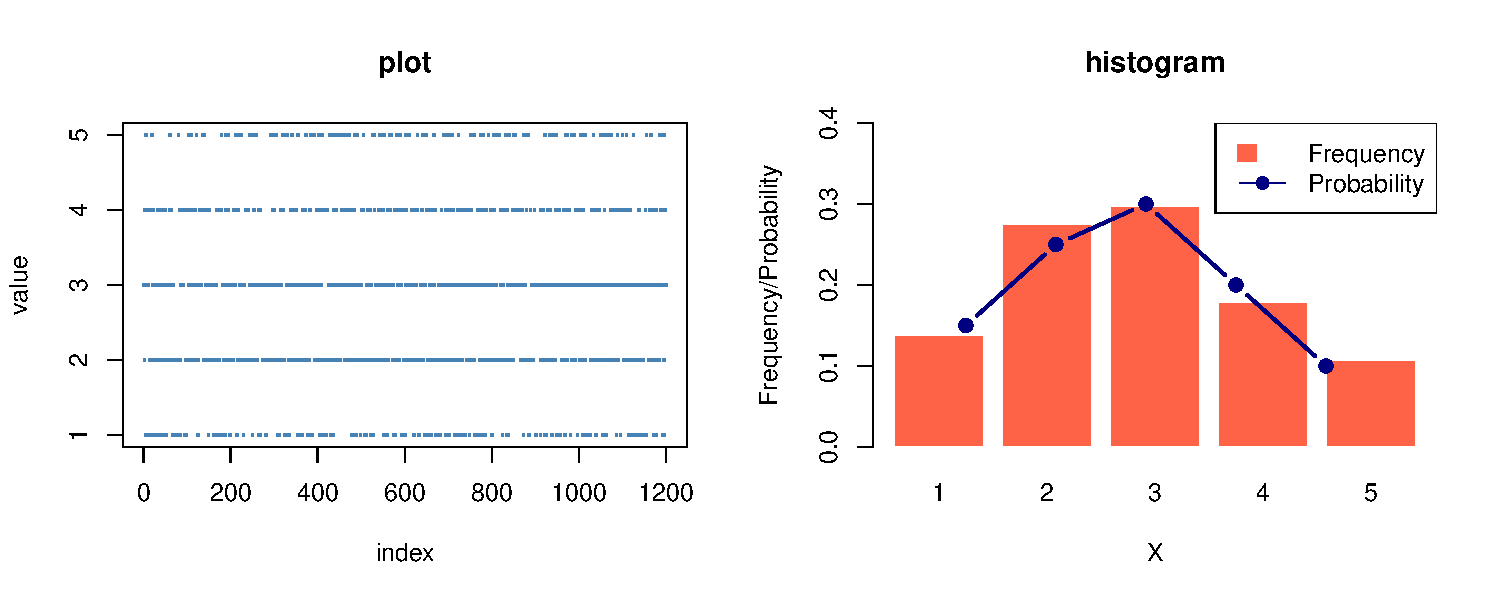
\includegraphics[keepaspectratio]{1_files/1_files/figure-latex/q1-1.pdf}}

\begin{Shaded}
\begin{Highlighting}[]
\FunctionTok{par}\NormalTok{(}\AttributeTok{mfrow =} \FunctionTok{c}\NormalTok{(}\DecValTok{1}\NormalTok{, }\DecValTok{1}\NormalTok{))}

\CommentTok{\# 数值对比}
\ControlFlowTok{for}\NormalTok{ (i }\ControlFlowTok{in} \FunctionTok{seq\_along}\NormalTok{(vals)) \{}
  \ControlFlowTok{if}\NormalTok{(i }\SpecialCharTok{==} \DecValTok{1}\NormalTok{) \{}
    \FunctionTok{cat}\NormalTok{(}\StringTok{"X}\SpecialCharTok{\textbackslash{}t}\StringTok{理论概率}\SpecialCharTok{\textbackslash{}t}\StringTok{观测频率}\SpecialCharTok{\textbackslash{}n}\StringTok{"}\NormalTok{)}
\NormalTok{  \}}
  \FunctionTok{cat}\NormalTok{(vals[i], }\StringTok{"}\SpecialCharTok{\textbackslash{}t}\StringTok{"}\NormalTok{, probs[i], }\StringTok{"}\SpecialCharTok{\textbackslash{}t\textbackslash{}t}\StringTok{"}\NormalTok{, }\FunctionTok{round}\NormalTok{(}\FunctionTok{mean}\NormalTok{(x }\SpecialCharTok{==}\NormalTok{ vals[i]), }\DecValTok{4}\NormalTok{), }\StringTok{"}\SpecialCharTok{\textbackslash{}n}\StringTok{"}\NormalTok{)}
\NormalTok{\}}
\end{Highlighting}
\end{Shaded}

\begin{verbatim}
## X    理论概率    观测频率
## 1     0.15        0.1392 
## 2     0.25        0.2758 
## 3     0.3         0.2975 
## 4     0.2         0.1792 
## 5     0.1         0.1083
\end{verbatim}

题目2:条件分布法与变换抽样法生成二维正态随机向量

\begin{Shaded}
\begin{Highlighting}[]
\FunctionTok{set.seed}\NormalTok{(}\DecValTok{2}\NormalTok{)}

\NormalTok{mu  }\OtherTok{\textless{}{-}} \FunctionTok{c}\NormalTok{(}\DecValTok{2}\NormalTok{, }\SpecialCharTok{{-}}\DecValTok{1}\NormalTok{)}
\NormalTok{Sig }\OtherTok{\textless{}{-}} \FunctionTok{matrix}\NormalTok{(}\FunctionTok{c}\NormalTok{(}\DecValTok{4}\NormalTok{, }\DecValTok{1}\NormalTok{, }\DecValTok{1}\NormalTok{, }\DecValTok{2}\NormalTok{), }\AttributeTok{nrow =} \DecValTok{2}\NormalTok{)}
\NormalTok{n2  }\OtherTok{\textless{}{-}} \DecValTok{1500}

\DocumentationTok{\#\# 方法一:条件分布法}
\DocumentationTok{\#\# X1 \textasciitilde{} N(mu1, s11);  X2|X1 \textasciitilde{} N(mu2 + s21/s11*(X1{-}mu1), s22 {-} s21\^{}2/s11)}
\NormalTok{x1\_cond }\OtherTok{\textless{}{-}} \FunctionTok{rnorm}\NormalTok{(n2, }\AttributeTok{mean =}\NormalTok{ mu[}\DecValTok{1}\NormalTok{], }\AttributeTok{sd =} \FunctionTok{sqrt}\NormalTok{(Sig[}\DecValTok{1}\NormalTok{,}\DecValTok{1}\NormalTok{]))}
\NormalTok{mu2\_cond }\OtherTok{\textless{}{-}}\NormalTok{ mu[}\DecValTok{2}\NormalTok{] }\SpecialCharTok{+}\NormalTok{ Sig[}\DecValTok{2}\NormalTok{,}\DecValTok{1}\NormalTok{]}\SpecialCharTok{/}\NormalTok{Sig[}\DecValTok{1}\NormalTok{,}\DecValTok{1}\NormalTok{] }\SpecialCharTok{*}\NormalTok{ (x1\_cond }\SpecialCharTok{{-}}\NormalTok{ mu[}\DecValTok{1}\NormalTok{])}
\NormalTok{s2\_cond  }\OtherTok{\textless{}{-}} \FunctionTok{sqrt}\NormalTok{(Sig[}\DecValTok{2}\NormalTok{,}\DecValTok{2}\NormalTok{] }\SpecialCharTok{{-}}\NormalTok{ Sig[}\DecValTok{2}\NormalTok{,}\DecValTok{1}\NormalTok{]}\SpecialCharTok{\^{}}\DecValTok{2}\SpecialCharTok{/}\NormalTok{Sig[}\DecValTok{1}\NormalTok{,}\DecValTok{1}\NormalTok{])}
\NormalTok{x2\_cond  }\OtherTok{\textless{}{-}} \FunctionTok{rnorm}\NormalTok{(n2, }\AttributeTok{mean =}\NormalTok{ mu2\_cond, }\AttributeTok{sd =}\NormalTok{ s2\_cond)}
\NormalTok{X\_cond   }\OtherTok{\textless{}{-}} \FunctionTok{cbind}\NormalTok{(x1\_cond, x2\_cond)}

\DocumentationTok{\#\# 方法二:变换抽样法(Cholesky 分解)}
\NormalTok{L   }\OtherTok{\textless{}{-}} \FunctionTok{t}\NormalTok{(}\FunctionTok{chol}\NormalTok{(Sig))              }\CommentTok{\# Sigma = L \%*\% t(L)}
\NormalTok{Z   }\OtherTok{\textless{}{-}} \FunctionTok{matrix}\NormalTok{(}\FunctionTok{rnorm}\NormalTok{(}\DecValTok{2} \SpecialCharTok{*}\NormalTok{ n2), }\AttributeTok{nrow =} \DecValTok{2}\NormalTok{)}
\NormalTok{X\_trans }\OtherTok{\textless{}{-}} \FunctionTok{t}\NormalTok{(L }\SpecialCharTok{\%*\%}\NormalTok{ Z }\SpecialCharTok{+}\NormalTok{ mu)      }\CommentTok{\# n2 x 2}

\FunctionTok{par}\NormalTok{(}\AttributeTok{mfrow =} \FunctionTok{c}\NormalTok{(}\DecValTok{1}\NormalTok{, }\DecValTok{2}\NormalTok{))}
\FunctionTok{plot}\NormalTok{(X\_cond,  }\AttributeTok{pch =} \StringTok{"."}\NormalTok{, }\AttributeTok{col =} \StringTok{"steelblue"}\NormalTok{,}
     \AttributeTok{main =} \StringTok{"Method1"}\NormalTok{, }\AttributeTok{xlab =} \StringTok{"X1"}\NormalTok{, }\AttributeTok{ylab =} \StringTok{"X2"}\NormalTok{)}
\FunctionTok{plot}\NormalTok{(X\_trans, }\AttributeTok{pch =} \StringTok{"."}\NormalTok{, }\AttributeTok{col =} \StringTok{"tomato"}\NormalTok{,}
     \AttributeTok{main =} \StringTok{"Method2"}\NormalTok{, }\AttributeTok{xlab =} \StringTok{"X1"}\NormalTok{, }\AttributeTok{ylab =} \StringTok{"X2"}\NormalTok{)}
\end{Highlighting}
\end{Shaded}

\pandocbounded{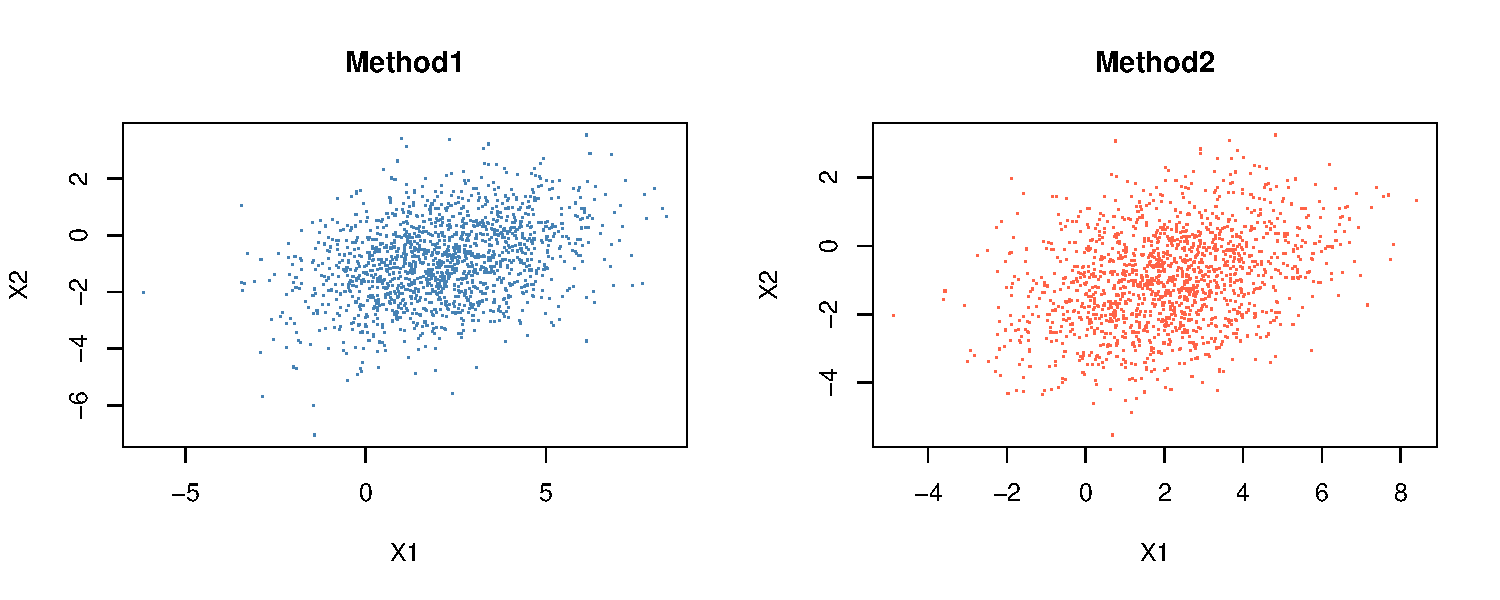
\includegraphics[keepaspectratio]{1_files/1_files/figure-latex/q2-1.pdf}}

\begin{Shaded}
\begin{Highlighting}[]
\FunctionTok{par}\NormalTok{(}\AttributeTok{mfrow =} \FunctionTok{c}\NormalTok{(}\DecValTok{1}\NormalTok{, }\DecValTok{1}\NormalTok{))}

\FunctionTok{cat}\NormalTok{(}\StringTok{"=== 条件分布法 ===}\SpecialCharTok{\textbackslash{}n}\StringTok{"}\NormalTok{,}
    \StringTok{"均值:"}\NormalTok{, }\FunctionTok{paste}\NormalTok{(}\FunctionTok{colMeans}\NormalTok{(X\_cond), }\AttributeTok{collapse =} \StringTok{" "}\NormalTok{), }\StringTok{"}\SpecialCharTok{\textbackslash{}n}\StringTok{"}\NormalTok{,}
    \StringTok{"协方差矩阵:}\SpecialCharTok{\textbackslash{}n}\StringTok{"}\NormalTok{,}
    \FunctionTok{paste}\NormalTok{(}\FunctionTok{capture.output}\NormalTok{(}\FunctionTok{cov}\NormalTok{(X\_cond)), }\AttributeTok{collapse =} \StringTok{"}\SpecialCharTok{\textbackslash{}n}\StringTok{"}\NormalTok{), }\StringTok{"}\SpecialCharTok{\textbackslash{}n}\StringTok{"}\NormalTok{)}
\end{Highlighting}
\end{Shaded}

\begin{verbatim}
## === 条件分布法 ===
##  均值: 2.10216820154314 -0.910444878145055 
##  协方差矩阵:
##            x1_cond   x2_cond
## x1_cond 3.9922889 0.9914779
## x2_cond 0.9914779 2.0653780
\end{verbatim}

\begin{Shaded}
\begin{Highlighting}[]
\FunctionTok{cat}\NormalTok{(}\StringTok{"=== 变换抽样法 ===}\SpecialCharTok{\textbackslash{}n}\StringTok{"}\NormalTok{,}
    \StringTok{"均值:"}\NormalTok{, }\FunctionTok{paste}\NormalTok{(}\FunctionTok{colMeans}\NormalTok{(X\_trans), }\AttributeTok{collapse =} \StringTok{" "}\NormalTok{), }\StringTok{"}\SpecialCharTok{\textbackslash{}n}\StringTok{"}\NormalTok{,}
    \StringTok{"协方差矩阵:}\SpecialCharTok{\textbackslash{}n}\StringTok{"}\NormalTok{,}
    \FunctionTok{paste}\NormalTok{(}\FunctionTok{capture.output}\NormalTok{(}\FunctionTok{cov}\NormalTok{(X\_trans)), }\AttributeTok{collapse =} \StringTok{"}\SpecialCharTok{\textbackslash{}n}\StringTok{"}\NormalTok{), }\StringTok{"}\SpecialCharTok{\textbackslash{}n}\StringTok{"}\NormalTok{)}
\end{Highlighting}
\end{Shaded}

\begin{verbatim}
## === 变换抽样法 ===
##  均值: 2.05776314220425 -0.981698674247148 
##  协方差矩阵:
##            [,1]      [,2]
## [1,] 3.7335413 0.8829907
## [2,] 0.8829907 1.9121234
\end{verbatim}

题目3:分层抽样习题2.5

\begin{Shaded}
\begin{Highlighting}[]
\CommentTok{\# r= 4层,各层大小 N=(20,30,25,25),总抽样量 m=10,重复1000次}
\FunctionTok{set.seed}\NormalTok{(}\DecValTok{3}\NormalTok{)}

\NormalTok{r      }\OtherTok{\textless{}{-}} \DecValTok{4}
\NormalTok{N\_strata }\OtherTok{\textless{}{-}} \FunctionTok{c}\NormalTok{(}\DecValTok{20}\NormalTok{, }\DecValTok{30}\NormalTok{, }\DecValTok{25}\NormalTok{, }\DecValTok{25}\NormalTok{)}
\NormalTok{N\_total  }\OtherTok{\textless{}{-}} \FunctionTok{sum}\NormalTok{(N\_strata)   }\CommentTok{\# 100}
\NormalTok{m        }\OtherTok{\textless{}{-}} \DecValTok{10}
\NormalTok{reps     }\OtherTok{\textless{}{-}} \DecValTok{1000}

\CommentTok{\# 按比例分配各层抽样量}
\NormalTok{m\_i }\OtherTok{\textless{}{-}} \FunctionTok{round}\NormalTok{(N\_strata }\SpecialCharTok{/}\NormalTok{ N\_total }\SpecialCharTok{*}\NormalTok{ m)}
\CommentTok{\# 如有舍入误差则修正到总量}
\NormalTok{m\_i[r] }\OtherTok{\textless{}{-}}\NormalTok{ m }\SpecialCharTok{{-}} \FunctionTok{sum}\NormalTok{(m\_i[}\SpecialCharTok{{-}}\NormalTok{r])}

\FunctionTok{cat}\NormalTok{(}\StringTok{"各层抽样量:"}\NormalTok{, m\_i, }\StringTok{"}\SpecialCharTok{\textbackslash{}n}\StringTok{"}\NormalTok{)}
\end{Highlighting}
\end{Shaded}

\begin{verbatim}
## 各层抽样量: 2 3 2 3
\end{verbatim}

\begin{Shaded}
\begin{Highlighting}[]
\CommentTok{\# 生成总体(用层编号标记)}
\NormalTok{population }\OtherTok{\textless{}{-}} \FunctionTok{rep}\NormalTok{(}\DecValTok{1}\SpecialCharTok{:}\NormalTok{r, }\AttributeTok{times =}\NormalTok{ N\_strata)}

\CommentTok{\# 重复1000次分层抽样}
\NormalTok{results }\OtherTok{\textless{}{-}} \FunctionTok{replicate}\NormalTok{(reps, \{}
\NormalTok{  sampled }\OtherTok{\textless{}{-}} \FunctionTok{c}\NormalTok{()}
  \ControlFlowTok{for}\NormalTok{ (k }\ControlFlowTok{in} \DecValTok{1}\SpecialCharTok{:}\NormalTok{r) \{}
\NormalTok{    pool }\OtherTok{\textless{}{-}} \FunctionTok{which}\NormalTok{(population }\SpecialCharTok{==}\NormalTok{ k)}
\NormalTok{    sampled }\OtherTok{\textless{}{-}} \FunctionTok{c}\NormalTok{(sampled, }\FunctionTok{sample}\NormalTok{(pool, m\_i[k]))}
\NormalTok{  \}}
\NormalTok{  sampled}
\NormalTok{\})}

\FunctionTok{cat}\NormalTok{(}\StringTok{"1000次抽样完成,每次抽"}\NormalTok{, m, }\StringTok{"个样本}\SpecialCharTok{\textbackslash{}n}\StringTok{"}\NormalTok{)}
\end{Highlighting}
\end{Shaded}

\begin{verbatim}
## 1000次抽样完成,每次抽 10 个样本
\end{verbatim}

\begin{Shaded}
\begin{Highlighting}[]
\FunctionTok{cat}\NormalTok{(}\StringTok{"前5次抽样结果(各取前3个编号):}\SpecialCharTok{\textbackslash{}n}\StringTok{"}\NormalTok{)}
\end{Highlighting}
\end{Shaded}

\begin{verbatim}
## 前5次抽样结果(各取前3个编号):
\end{verbatim}

\begin{Shaded}
\begin{Highlighting}[]
\FunctionTok{print}\NormalTok{(results[}\DecValTok{1}\SpecialCharTok{:}\DecValTok{3}\NormalTok{, }\DecValTok{1}\SpecialCharTok{:}\DecValTok{5}\NormalTok{])}
\end{Highlighting}
\end{Shaded}

\begin{verbatim}
##      [,1] [,2] [,3] [,4] [,5]
## [1,]    5    8    5   19    8
## [2,]   12   16    9    6   10
## [3,]   27   28   29   28   24
\end{verbatim}

\begin{Shaded}
\begin{Highlighting}[]
\CommentTok{\# 各层被抽到频率}
\NormalTok{layer\_freq }\OtherTok{\textless{}{-}} \FunctionTok{apply}\NormalTok{(results, }\DecValTok{2}\NormalTok{, }\ControlFlowTok{function}\NormalTok{(s) }\FunctionTok{table}\NormalTok{(}\FunctionTok{factor}\NormalTok{(population[s], }\AttributeTok{levels=}\DecValTok{1}\SpecialCharTok{:}\NormalTok{r)))}
\FunctionTok{cat}\NormalTok{(}\StringTok{"各层平均被抽频率:}\SpecialCharTok{\textbackslash{}n}\StringTok{"}\NormalTok{)}
\end{Highlighting}
\end{Shaded}

\begin{verbatim}
## 各层平均被抽频率:
\end{verbatim}

\begin{Shaded}
\begin{Highlighting}[]
\FunctionTok{print}\NormalTok{(}\FunctionTok{round}\NormalTok{(}\FunctionTok{rowMeans}\NormalTok{(layer\_freq) }\SpecialCharTok{/}\NormalTok{ m, }\DecValTok{3}\NormalTok{))}
\end{Highlighting}
\end{Shaded}

\begin{verbatim}
##   1   2   3   4 
## 0.2 0.3 0.2 0.3
\end{verbatim}

\begin{Shaded}
\begin{Highlighting}[]
\FunctionTok{cat}\NormalTok{(}\StringTok{"理论各层抽取比例:"}\NormalTok{, N\_strata }\SpecialCharTok{/}\NormalTok{ N\_total, }\StringTok{"}\SpecialCharTok{\textbackslash{}n}\StringTok{"}\NormalTok{)}
\end{Highlighting}
\end{Shaded}

\begin{verbatim}
## 理论各层抽取比例: 0.2 0.3 0.25 0.25
\end{verbatim}

题目4:泊松分布参数的期望与方差估计(\(\lambda=3\),n=800,重复2000次)

\begin{Shaded}
\begin{Highlighting}[]
\FunctionTok{set.seed}\NormalTok{(}\DecValTok{4}\NormalTok{)}

\NormalTok{lambda\_true }\OtherTok{\textless{}{-}} \DecValTok{3}
\NormalTok{n4          }\OtherTok{\textless{}{-}} \DecValTok{800}
\NormalTok{reps4       }\OtherTok{\textless{}{-}} \DecValTok{2000}

\CommentTok{\# 估计量:lambda\_hat = X\_bar(同时估计期望与方差)}
\NormalTok{sim }\OtherTok{\textless{}{-}} \FunctionTok{replicate}\NormalTok{(reps4, \{}
\NormalTok{  x      }\OtherTok{\textless{}{-}} \FunctionTok{rpois}\NormalTok{(n4, }\AttributeTok{lambda =}\NormalTok{ lambda\_true)}
\NormalTok{  lambda\_hat }\OtherTok{\textless{}{-}} \FunctionTok{mean}\NormalTok{(x)      }\CommentTok{\# MLE = 矩估计 = 样本均值}
\NormalTok{  var\_hat    }\OtherTok{\textless{}{-}} \FunctionTok{var}\NormalTok{(x)       }\CommentTok{\# 样本方差}
  \FunctionTok{c}\NormalTok{(lambda\_hat, var\_hat)}
\NormalTok{\})}

\NormalTok{lambda\_ests }\OtherTok{\textless{}{-}}\NormalTok{ sim[}\DecValTok{1}\NormalTok{, ]}
\NormalTok{var\_ests    }\OtherTok{\textless{}{-}}\NormalTok{ sim[}\DecValTok{2}\NormalTok{, ]}

\FunctionTok{cat}\NormalTok{(}\StringTok{"=== 期望估计(lambda\_hat = X\_bar)===}\SpecialCharTok{\textbackslash{}n}\StringTok{"}\NormalTok{)}
\end{Highlighting}
\end{Shaded}

\begin{verbatim}
## === 期望估计(lambda_hat = X_bar)===
\end{verbatim}

\begin{Shaded}
\begin{Highlighting}[]
\FunctionTok{cat}\NormalTok{(}\StringTok{"真实值 lambda=3}\SpecialCharTok{\textbackslash{}n}\StringTok{"}\NormalTok{)}
\end{Highlighting}
\end{Shaded}

\begin{verbatim}
## 真实值 lambda=3
\end{verbatim}

\begin{Shaded}
\begin{Highlighting}[]
\FunctionTok{cat}\NormalTok{(}\StringTok{"估计均值:"}\NormalTok{, }\FunctionTok{round}\NormalTok{(}\FunctionTok{mean}\NormalTok{(lambda\_ests), }\DecValTok{4}\NormalTok{), }\StringTok{"}\SpecialCharTok{\textbackslash{}n}\StringTok{"}\NormalTok{)}
\end{Highlighting}
\end{Shaded}

\begin{verbatim}
## 估计均值: 3.0007
\end{verbatim}

\begin{Shaded}
\begin{Highlighting}[]
\FunctionTok{cat}\NormalTok{(}\StringTok{"估计标准差:"}\NormalTok{, }\FunctionTok{round}\NormalTok{(}\FunctionTok{sd}\NormalTok{(lambda\_ests), }\DecValTok{4}\NormalTok{), }\StringTok{"}\SpecialCharTok{\textbackslash{}n}\StringTok{"}\NormalTok{)}
\end{Highlighting}
\end{Shaded}

\begin{verbatim}
## 估计标准差: 0.0621
\end{verbatim}

\begin{Shaded}
\begin{Highlighting}[]
\FunctionTok{cat}\NormalTok{(}\StringTok{"理论标准误 sqrt(lambda/n):"}\NormalTok{, }\FunctionTok{round}\NormalTok{(}\FunctionTok{sqrt}\NormalTok{(lambda\_true}\SpecialCharTok{/}\NormalTok{n4), }\DecValTok{4}\NormalTok{), }\StringTok{"}\SpecialCharTok{\textbackslash{}n\textbackslash{}n}\StringTok{"}\NormalTok{)}
\end{Highlighting}
\end{Shaded}

\begin{verbatim}
## 理论标准误 sqrt(lambda/n): 0.0612
\end{verbatim}

\begin{Shaded}
\begin{Highlighting}[]
\FunctionTok{cat}\NormalTok{(}\StringTok{"=== 方差估计(S\^{}2)===}\SpecialCharTok{\textbackslash{}n}\StringTok{"}\NormalTok{)}
\end{Highlighting}
\end{Shaded}

\begin{verbatim}
## === 方差估计(S^2)===
\end{verbatim}

\begin{Shaded}
\begin{Highlighting}[]
\FunctionTok{cat}\NormalTok{(}\StringTok{"真实值 Var(X)=lambda=3}\SpecialCharTok{\textbackslash{}n}\StringTok{"}\NormalTok{)}
\end{Highlighting}
\end{Shaded}

\begin{verbatim}
## 真实值 Var(X)=lambda=3
\end{verbatim}

\begin{Shaded}
\begin{Highlighting}[]
\FunctionTok{cat}\NormalTok{(}\StringTok{"估计均值:"}\NormalTok{, }\FunctionTok{round}\NormalTok{(}\FunctionTok{mean}\NormalTok{(var\_ests), }\DecValTok{4}\NormalTok{), }\StringTok{"}\SpecialCharTok{\textbackslash{}n}\StringTok{"}\NormalTok{)}
\end{Highlighting}
\end{Shaded}

\begin{verbatim}
## 估计均值: 2.9982
\end{verbatim}

\begin{Shaded}
\begin{Highlighting}[]
\FunctionTok{cat}\NormalTok{(}\StringTok{"估计标准差:"}\NormalTok{, }\FunctionTok{round}\NormalTok{(}\FunctionTok{sd}\NormalTok{(var\_ests), }\DecValTok{4}\NormalTok{), }\StringTok{"}\SpecialCharTok{\textbackslash{}n}\StringTok{"}\NormalTok{)}
\end{Highlighting}
\end{Shaded}

\begin{verbatim}
## 估计标准差: 0.1632
\end{verbatim}

\begin{Shaded}
\begin{Highlighting}[]
\FunctionTok{par}\NormalTok{(}\AttributeTok{mfrow =} \FunctionTok{c}\NormalTok{(}\DecValTok{1}\NormalTok{, }\DecValTok{2}\NormalTok{))}
\FunctionTok{hist}\NormalTok{(lambda\_ests, }\AttributeTok{breaks =} \DecValTok{40}\NormalTok{, }\AttributeTok{col =} \StringTok{"steelblue"}\NormalTok{, }\AttributeTok{border =} \StringTok{"white"}\NormalTok{,}
     \AttributeTok{main =} \StringTok{"Distribution of Lambda Hat"}\NormalTok{, }\AttributeTok{xlab =} \StringTok{"lambda\_hat"}\NormalTok{)}
\FunctionTok{abline}\NormalTok{(}\AttributeTok{v =}\NormalTok{ lambda\_true, }\AttributeTok{col =} \StringTok{"red"}\NormalTok{, }\AttributeTok{lwd =} \DecValTok{2}\NormalTok{)}

\FunctionTok{hist}\NormalTok{(var\_ests, }\AttributeTok{breaks =} \DecValTok{40}\NormalTok{, }\AttributeTok{col =} \StringTok{"tomato"}\NormalTok{, }\AttributeTok{border =} \StringTok{"white"}\NormalTok{,}
     \AttributeTok{main =} \StringTok{"Distribution of Variance Estimate"}\NormalTok{, }\AttributeTok{xlab =} \StringTok{"S\^{}2"}\NormalTok{)}
\FunctionTok{abline}\NormalTok{(}\AttributeTok{v =}\NormalTok{ lambda\_true, }\AttributeTok{col =} \StringTok{"navy"}\NormalTok{, }\AttributeTok{lwd =} \DecValTok{2}\NormalTok{)}
\end{Highlighting}
\end{Shaded}

\pandocbounded{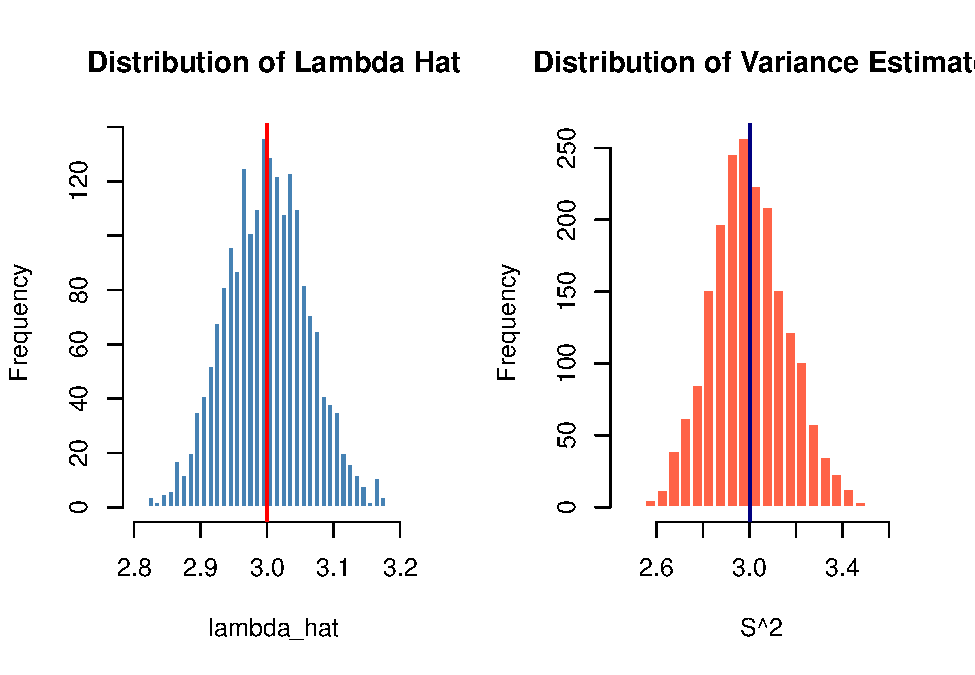
\includegraphics[keepaspectratio]{1_files/1_files/figure-latex/q4-1.pdf}}

\begin{Shaded}
\begin{Highlighting}[]
\FunctionTok{par}\NormalTok{(}\AttributeTok{mfrow =} \FunctionTok{c}\NormalTok{(}\DecValTok{1}\NormalTok{, }\DecValTok{1}\NormalTok{))}
\end{Highlighting}
\end{Shaded}

题目5:Power分布 \(f(x;\alpha)=\alpha x^{\alpha-1}, 0<x<1\)
\(n=600, \alpha=0.5\):矩估计 vs MLE,比较MSE

\begin{Shaded}
\begin{Highlighting}[]
\FunctionTok{set.seed}\NormalTok{(}\DecValTok{5}\NormalTok{)}

\NormalTok{alpha\_true }\OtherTok{\textless{}{-}} \FloatTok{0.5}
\NormalTok{n5         }\OtherTok{\textless{}{-}} \DecValTok{600}
\NormalTok{reps5      }\OtherTok{\textless{}{-}} \DecValTok{2000}

\CommentTok{\# 生成 Power(alpha) 随机数:U\^{}(1/alpha)}
\NormalTok{sim5 }\OtherTok{\textless{}{-}} \FunctionTok{replicate}\NormalTok{(reps5, \{}
\NormalTok{  u }\OtherTok{\textless{}{-}} \FunctionTok{runif}\NormalTok{(n5)}
\NormalTok{  x }\OtherTok{\textless{}{-}}\NormalTok{ u}\SpecialCharTok{\^{}}\NormalTok{(}\DecValTok{1}\SpecialCharTok{/}\NormalTok{alpha\_true)}

  \CommentTok{\# 矩估计:E[X]=alpha/(alpha+1) =\textgreater{} alpha\_mom = X\_bar/(1{-}X\_bar)}
\NormalTok{  xbar     }\OtherTok{\textless{}{-}} \FunctionTok{mean}\NormalTok{(x)}
\NormalTok{  alpha\_mom }\OtherTok{\textless{}{-}}\NormalTok{ xbar }\SpecialCharTok{/}\NormalTok{ (}\DecValTok{1} \SpecialCharTok{{-}}\NormalTok{ xbar)}

  \CommentTok{\# MLE:alpha\_mle = {-}n / sum(log(x))}
\NormalTok{  alpha\_mle }\OtherTok{\textless{}{-}} \SpecialCharTok{{-}}\NormalTok{n5 }\SpecialCharTok{/} \FunctionTok{sum}\NormalTok{(}\FunctionTok{log}\NormalTok{(x))}

  \FunctionTok{c}\NormalTok{(alpha\_mom, alpha\_mle)}
\NormalTok{\})}

\NormalTok{mom\_ests }\OtherTok{\textless{}{-}}\NormalTok{ sim5[}\DecValTok{1}\NormalTok{, ]}
\NormalTok{mle\_ests }\OtherTok{\textless{}{-}}\NormalTok{ sim5[}\DecValTok{2}\NormalTok{, ]}

\NormalTok{mse\_mom }\OtherTok{\textless{}{-}} \FunctionTok{mean}\NormalTok{((mom\_ests }\SpecialCharTok{{-}}\NormalTok{ alpha\_true)}\SpecialCharTok{\^{}}\DecValTok{2}\NormalTok{)}
\NormalTok{mse\_mle }\OtherTok{\textless{}{-}} \FunctionTok{mean}\NormalTok{((mle\_ests }\SpecialCharTok{{-}}\NormalTok{ alpha\_true)}\SpecialCharTok{\^{}}\DecValTok{2}\NormalTok{)}

\FunctionTok{cat}\NormalTok{(}\StringTok{"=== 矩估计 ===}\SpecialCharTok{\textbackslash{}n}\StringTok{"}\NormalTok{)}
\end{Highlighting}
\end{Shaded}

\begin{verbatim}
## === 矩估计 ===
\end{verbatim}

\begin{Shaded}
\begin{Highlighting}[]
\FunctionTok{cat}\NormalTok{(}\StringTok{"均值:"}\NormalTok{, }\FunctionTok{round}\NormalTok{(}\FunctionTok{mean}\NormalTok{(mom\_ests), }\DecValTok{4}\NormalTok{),}
    \StringTok{" 偏差:"}\NormalTok{, }\FunctionTok{round}\NormalTok{(}\FunctionTok{mean}\NormalTok{(mom\_ests) }\SpecialCharTok{{-}}\NormalTok{ alpha\_true, }\DecValTok{4}\NormalTok{),}
    \StringTok{" MSE:"}\NormalTok{, }\FunctionTok{round}\NormalTok{(mse\_mom, }\DecValTok{6}\NormalTok{), }\StringTok{"}\SpecialCharTok{\textbackslash{}n\textbackslash{}n}\StringTok{"}\NormalTok{)}
\end{Highlighting}
\end{Shaded}

\begin{verbatim}
## 均值: 0.4994  偏差: -6e-04  MSE: 0.000736
\end{verbatim}

\begin{Shaded}
\begin{Highlighting}[]
\FunctionTok{cat}\NormalTok{(}\StringTok{"=== 最大似然估计 ===}\SpecialCharTok{\textbackslash{}n}\StringTok{"}\NormalTok{)}
\end{Highlighting}
\end{Shaded}

\begin{verbatim}
## === 最大似然估计 ===
\end{verbatim}

\begin{Shaded}
\begin{Highlighting}[]
\FunctionTok{cat}\NormalTok{(}\StringTok{"均值:"}\NormalTok{, }\FunctionTok{round}\NormalTok{(}\FunctionTok{mean}\NormalTok{(mle\_ests), }\DecValTok{4}\NormalTok{),}
    \StringTok{" 偏差:"}\NormalTok{, }\FunctionTok{round}\NormalTok{(}\FunctionTok{mean}\NormalTok{(mle\_ests) }\SpecialCharTok{{-}}\NormalTok{ alpha\_true, }\DecValTok{4}\NormalTok{),}
    \StringTok{" MSE:"}\NormalTok{, }\FunctionTok{round}\NormalTok{(mse\_mle, }\DecValTok{6}\NormalTok{), }\StringTok{"}\SpecialCharTok{\textbackslash{}n}\StringTok{"}\NormalTok{)}
\end{Highlighting}
\end{Shaded}

\begin{verbatim}
## 均值: 0.4999  偏差: -1e-04  MSE: 0.000408
\end{verbatim}

\begin{Shaded}
\begin{Highlighting}[]
\FunctionTok{cat}\NormalTok{(}\StringTok{"}\SpecialCharTok{\textbackslash{}n}\StringTok{MSE之比 (MOM/MLE):"}\NormalTok{, }\FunctionTok{round}\NormalTok{(mse\_mom}\SpecialCharTok{/}\NormalTok{mse\_mle, }\DecValTok{4}\NormalTok{), }\StringTok{"}\SpecialCharTok{\textbackslash{}n}\StringTok{"}\NormalTok{)}
\end{Highlighting}
\end{Shaded}

\begin{verbatim}
## 
## MSE之比 (MOM/MLE): 1.8066
\end{verbatim}

题目6:线性模型 \(Y = \alpha + \beta*X + \epsilon,\alpha=2,\beta=1.5\)
\(X~U(0,1),\epsilon~N(0,1)\),500组样本,OLS估计

\begin{Shaded}
\begin{Highlighting}[]
\FunctionTok{set.seed}\NormalTok{(}\DecValTok{6}\NormalTok{)}

\NormalTok{alpha\_true }\OtherTok{\textless{}{-}} \DecValTok{2}
\NormalTok{beta\_true  }\OtherTok{\textless{}{-}} \FloatTok{1.5}
\NormalTok{n6         }\OtherTok{\textless{}{-}} \DecValTok{500}

\NormalTok{X   }\OtherTok{\textless{}{-}} \FunctionTok{runif}\NormalTok{(n6, }\DecValTok{0}\NormalTok{, }\DecValTok{1}\NormalTok{)}
\NormalTok{eps }\OtherTok{\textless{}{-}} \FunctionTok{rnorm}\NormalTok{(n6, }\DecValTok{0}\NormalTok{, }\DecValTok{1}\NormalTok{)}
\NormalTok{Y   }\OtherTok{\textless{}{-}}\NormalTok{ alpha\_true }\SpecialCharTok{+}\NormalTok{ beta\_true }\SpecialCharTok{*}\NormalTok{ X }\SpecialCharTok{+}\NormalTok{ eps}

\CommentTok{\# OLS 最小二乘估计}
\NormalTok{Xmat }\OtherTok{\textless{}{-}} \FunctionTok{cbind}\NormalTok{(}\DecValTok{1}\NormalTok{, X)}
\NormalTok{coef\_ols }\OtherTok{\textless{}{-}} \FunctionTok{solve}\NormalTok{(}\FunctionTok{t}\NormalTok{(Xmat) }\SpecialCharTok{\%*\%}\NormalTok{ Xmat) }\SpecialCharTok{\%*\%} \FunctionTok{t}\NormalTok{(Xmat) }\SpecialCharTok{\%*\%}\NormalTok{ Y}

\NormalTok{alpha\_hat }\OtherTok{\textless{}{-}}\NormalTok{ coef\_ols[}\DecValTok{1}\NormalTok{]}
\NormalTok{beta\_hat  }\OtherTok{\textless{}{-}}\NormalTok{ coef\_ols[}\DecValTok{2}\NormalTok{]}

\FunctionTok{cat}\NormalTok{(}\StringTok{"真实值:alpha="}\NormalTok{, alpha\_true, }\StringTok{" beta="}\NormalTok{, beta\_true, }\StringTok{"}\SpecialCharTok{\textbackslash{}n}\StringTok{"}\NormalTok{)}
\end{Highlighting}
\end{Shaded}

\begin{verbatim}
## 真实值:alpha= 2  beta= 1.5
\end{verbatim}

\begin{Shaded}
\begin{Highlighting}[]
\FunctionTok{cat}\NormalTok{(}\StringTok{"OLS估计:alpha\_hat="}\NormalTok{, }\FunctionTok{round}\NormalTok{(alpha\_hat, }\DecValTok{4}\NormalTok{),}
    \StringTok{" beta\_hat="}\NormalTok{, }\FunctionTok{round}\NormalTok{(beta\_hat, }\DecValTok{4}\NormalTok{), }\StringTok{"}\SpecialCharTok{\textbackslash{}n}\StringTok{"}\NormalTok{)}
\end{Highlighting}
\end{Shaded}

\begin{verbatim}
## OLS估计:alpha_hat= 2.0556  beta_hat= 1.3421
\end{verbatim}

\begin{Shaded}
\begin{Highlighting}[]
\CommentTok{\# 与 lm() 结果对比}
\NormalTok{fit }\OtherTok{\textless{}{-}} \FunctionTok{lm}\NormalTok{(Y }\SpecialCharTok{\textasciitilde{}}\NormalTok{ X)}
\FunctionTok{cat}\NormalTok{(}\StringTok{"}\SpecialCharTok{\textbackslash{}n}\StringTok{lm() 验证:}\SpecialCharTok{\textbackslash{}n}\StringTok{"}\NormalTok{); }\FunctionTok{print}\NormalTok{(}\FunctionTok{coef}\NormalTok{(fit))}
\end{Highlighting}
\end{Shaded}

\begin{verbatim}
## 
## lm() 验证:
\end{verbatim}

\begin{verbatim}
## (Intercept)           X 
##    2.055588    1.342114
\end{verbatim}

\begin{Shaded}
\begin{Highlighting}[]
\CommentTok{\# 散点图 + 拟合线}
\FunctionTok{plot}\NormalTok{(X, Y, }\AttributeTok{pch =} \StringTok{"."}\NormalTok{, }\AttributeTok{col =} \StringTok{"gray50"}\NormalTok{,}
     \AttributeTok{main =} \StringTok{"线性模型 OLS 拟合(n=500)"}\NormalTok{,}
     \AttributeTok{xlab =} \StringTok{"X"}\NormalTok{, }\AttributeTok{ylab =} \StringTok{"Y"}\NormalTok{)}
\FunctionTok{abline}\NormalTok{(}\AttributeTok{a =}\NormalTok{ alpha\_true, }\AttributeTok{b =}\NormalTok{ beta\_true, }\AttributeTok{col =} \StringTok{"navy"}\NormalTok{,  }\AttributeTok{lwd =} \DecValTok{2}\NormalTok{, }\AttributeTok{lty =} \DecValTok{2}\NormalTok{)}
\FunctionTok{abline}\NormalTok{(}\AttributeTok{a =}\NormalTok{ alpha\_hat,  }\AttributeTok{b =}\NormalTok{ beta\_hat,  }\AttributeTok{col =} \StringTok{"tomato"}\NormalTok{, }\AttributeTok{lwd =} \DecValTok{2}\NormalTok{)}
\FunctionTok{legend}\NormalTok{(}\StringTok{"topleft"}\NormalTok{,}
       \AttributeTok{legend =} \FunctionTok{c}\NormalTok{(}\StringTok{"真实直线"}\NormalTok{, }\StringTok{"OLS估计"}\NormalTok{),}
       \AttributeTok{col    =} \FunctionTok{c}\NormalTok{(}\StringTok{"navy"}\NormalTok{, }\StringTok{"tomato"}\NormalTok{),}
       \AttributeTok{lty    =} \FunctionTok{c}\NormalTok{(}\DecValTok{2}\NormalTok{, }\DecValTok{1}\NormalTok{), }\AttributeTok{lwd =} \DecValTok{2}\NormalTok{)}
\end{Highlighting}
\end{Shaded}

\pandocbounded{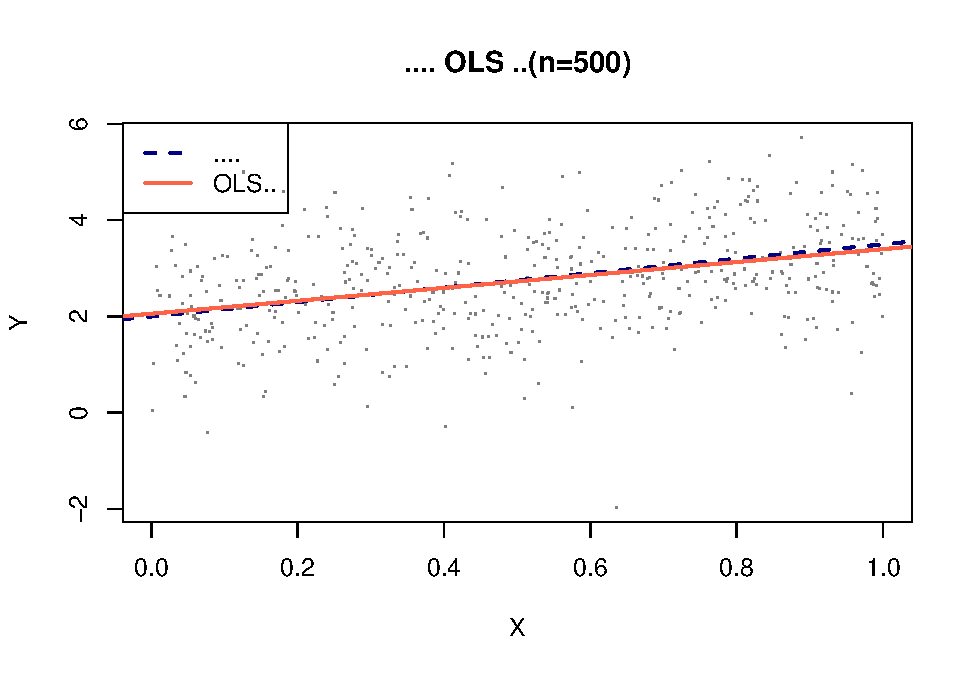
\includegraphics[keepaspectratio]{1_files/1_files/figure-latex/q6-1.pdf}}

\section{============================================================}\label{section}

\section{课堂作业(iris 散点图 \&
均匀分布直方图)}\label{ux8bfeux5802ux4f5cux4e1airis-ux6563ux70b9ux56fe-ux5747ux5300ux5206ux5e03ux76f4ux65b9ux56fe}

\section{============================================================}\label{section-1}

\begin{Shaded}
\begin{Highlighting}[]
\CommentTok{\# iris 花瓣长度与宽度散点图}
\NormalTok{colors }\OtherTok{\textless{}{-}} \FunctionTok{c}\NormalTok{(}\StringTok{"setosa"} \OtherTok{=} \StringTok{"tomato"}\NormalTok{, }\StringTok{"versicolor"} \OtherTok{=} \StringTok{"steelblue"}\NormalTok{, }\StringTok{"virginica"} \OtherTok{=} \StringTok{"seagreen"}\NormalTok{)}

\FunctionTok{plot}\NormalTok{(Petal.Width }\SpecialCharTok{\textasciitilde{}}\NormalTok{ Petal.Length,}
     \AttributeTok{data  =}\NormalTok{ iris,}
     \AttributeTok{col   =}\NormalTok{ colors[}\FunctionTok{as.character}\NormalTok{(iris}\SpecialCharTok{$}\NormalTok{Species)],}
     \AttributeTok{pch   =} \DecValTok{19}\NormalTok{,}
     \AttributeTok{cex   =} \FloatTok{0.8}\NormalTok{,}
     \AttributeTok{main  =} \StringTok{"Iris"}\NormalTok{,}
     \AttributeTok{xlim  =} \FunctionTok{c}\NormalTok{(}\DecValTok{1}\NormalTok{, }\DecValTok{7}\NormalTok{),}
     \AttributeTok{ylim  =} \FunctionTok{c}\NormalTok{(}\DecValTok{0}\NormalTok{, }\DecValTok{4}\NormalTok{),}
     \AttributeTok{xlab  =} \StringTok{"Petal Length"}\NormalTok{,}
     \AttributeTok{ylab  =} \StringTok{"Petal Width"}\NormalTok{)}

\FunctionTok{legend}\NormalTok{(}\StringTok{"topright"}\NormalTok{,}
       \AttributeTok{legend =} \FunctionTok{names}\NormalTok{(colors),}
       \AttributeTok{col    =}\NormalTok{ colors,}
       \AttributeTok{pch    =} \DecValTok{19}\NormalTok{,}
       \AttributeTok{title  =} \StringTok{"Species"}\NormalTok{)}
\end{Highlighting}
\end{Shaded}

\pandocbounded{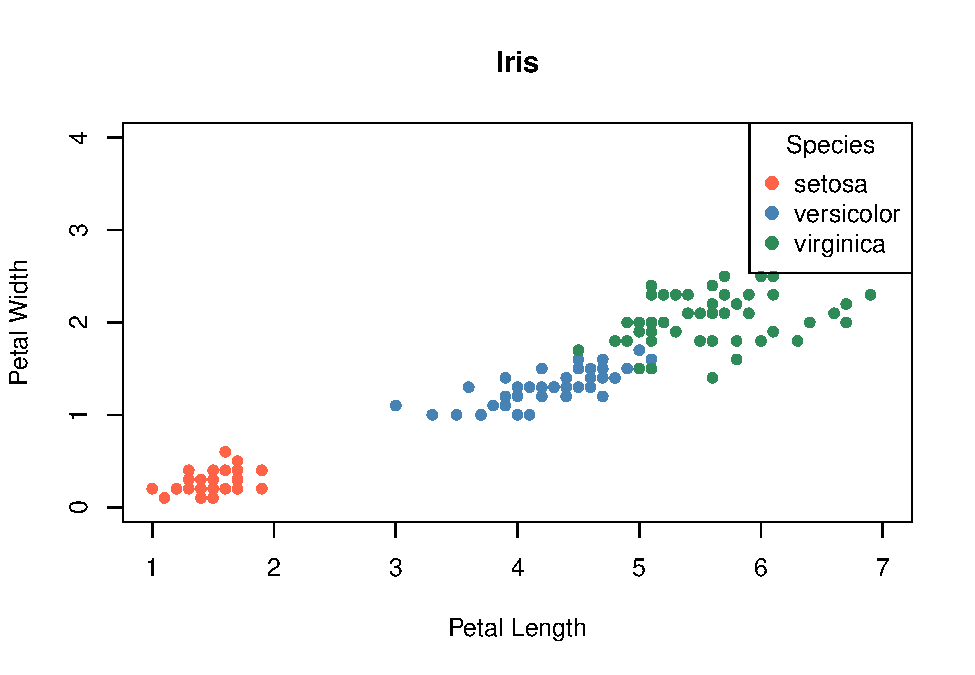
\includegraphics[keepaspectratio]{1_files/1_files/figure-latex/iris_plot-1.pdf}}

\begin{Shaded}
\begin{Highlighting}[]
\CommentTok{\# 生成 [0, 10] 之间 100 个均匀分布随机数}
\FunctionTok{set.seed}\NormalTok{(}\DecValTok{42}\NormalTok{)}
\NormalTok{x }\OtherTok{\textless{}{-}} \FunctionTok{runif}\NormalTok{(}\DecValTok{100}\NormalTok{, }\AttributeTok{min =} \DecValTok{0}\NormalTok{, }\AttributeTok{max =} \DecValTok{10}\NormalTok{)}

\CommentTok{\# 频数直方图}
\FunctionTok{hist}\NormalTok{(x,}
     \AttributeTok{main  =} \StringTok{"title\_1"}\NormalTok{,}
     \AttributeTok{xlab  =} \StringTok{"value"}\NormalTok{,}
     \AttributeTok{ylab  =} \StringTok{"count"}\NormalTok{,}
     \AttributeTok{col   =} \StringTok{"steelblue"}\NormalTok{,}
     \AttributeTok{border =} \StringTok{"white"}\NormalTok{)}
\end{Highlighting}
\end{Shaded}

\pandocbounded{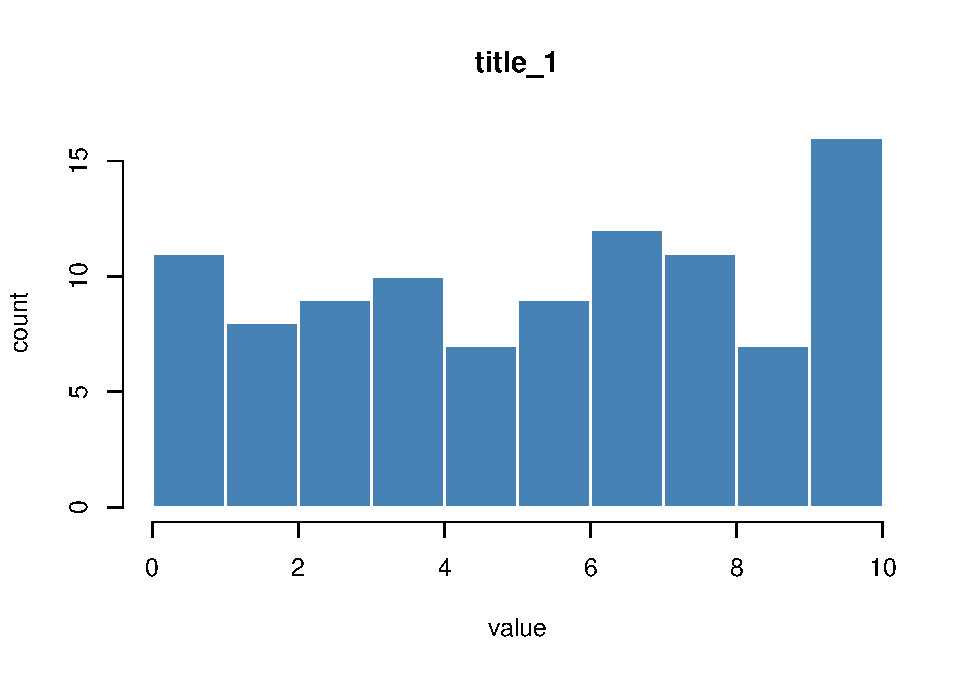
\includegraphics[keepaspectratio]{1_files/1_files/figure-latex/unnamed-chunk-1-1.pdf}}

\end{document}
